%%%%%%%%%%%%%%%%%%%%%%%%%%%%%%%%%%%%%%%%%%%%%%%%%%%%%%%%%%%%%%%%%%%%%
%
% talk intro optimization Cotonou 2022
%
%%%%%%%%%%%%%%%%%%%%%%%%%%%%%%%%%%%%%%%%%%%%%%%%%%%%%%%%%%%%%%%%%%%%%

\documentclass[12pt]{beamer}
\usepackage[utf8]{inputenc}
\usepackage{amsmath}
\usepackage{amsfonts}
\usepackage{amssymb}
\usepackage{graphicx}
\graphicspath{{figures/}{Figures/}}
%\usepackage{beamerthemesplit}
%\usepackage{beamerthemeshadow} 
\usepackage{color}
\usepackage{hyperref}
\usepackage{xspace}
\usepackage{xifthen}
\usepackage{multicol}
\usepackage{mathtools}
\usepackage{algorithm,algorithmicx}
\usepackage{algcompatible}
\usepackage{bbm}
\usepackage{textcomp}
\usepackage{yfonts}

\usepackage{tikz}
\usetikzlibrary{calc,shapes,arrows}

% custom commands in sty file, for easier writting and change of notations
\usepackage{my_notations}
\newcommand*{\mmds}{\enm{\text{MMD}^2}}

\usetheme{Madrid}
\usecolortheme{beaver}

%%%%%%%%%%%%%%%%%%%%%%%%%%%%%%%%%%%%%%%%%%%%%%%%%%%%%%%%%%%%%%%%%%%%%
\begin{document}
\title
[Optimization: multi-tasker or utopia?
%\hspace{0.1cm} \insertframenumber/\inserttotalframenumber
]
{Optimization for quantitative decisions: a versatile multi-tasker or an utopia?}
\author
[R. Le Riche]
{\large Rodolphe Le Riche$^{*}$}
\institute[CNRS LIMOS]{$^*$~CNRS at LIMOS (Mines Saint Etienne, UCA) France
} 
\date[July 2022]{25 July 2022 \\
Cotonou, Benin, IA summer school 
\\\vskip\baselineskip
{\small Acknowledgements : Vallet foundation, Bernard Guy}
} 
\begin{frame}
\titlepage
\end{frame}

%=======================================================================================
\begin{frame}
\frametitle{Abstract} 
{\footnotesize
The study of optimization algorithms started at the end of World War II and has since then experienced a constantly growing interest, fueled by needs in engineering, computational simulation and Machine Learning.
In this talk, we look into the history of the new scientific objects that are the optimizers. 
The point-of-view is historical and philosophical rather than mathematical.
It is explained how the conditions for the emergence of the optimizers as new scientific objects correspond to a state of sufficient knowledge decomposition. 
The versatility of optimizers is illustrated through examples.
Although they are just tools, optimizers are a source a fascination because they guide through a space of representations in a process that resembles learning. 
But rationality is bounded and, in that sense, optimization problems are utopias: they are an over-simplification of decisions which are actually rooted in human relationships; they often cannot be solved because the computational capacities are limited.  
The presentation finishes with some contemporary challenges in optimization.
}
\end{frame}

%=======================================================================================
%\begin{frame}[allowframebreaks]
%\frametitle{Content} 
%\begin{multicols}{2}
%\tableofcontents[currentsection]
%\end{multicols}
%\end{frame}


%=======================================================================================
\begin{frame}[allowframebreaks]
\frametitle{The advent of optimization algorithms}
\begin{minipage}[b]{0.25\textwidth}
\centering
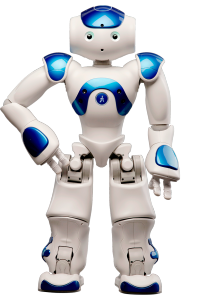
\includegraphics[width=0.4\textwidth]{Figures/NAO.png}
\\ ``Intelligence'' =
\end{minipage} 
\hfill
\begin{minipage}[b]{0.2\textwidth}
{\scriptsize \cite{bachoptimization}}
\vskip 2cm
~
\end{minipage} 
\\
\hfill
\begin{minipage}[t]{0.2\textwidth}
\centering
 models + 
\\
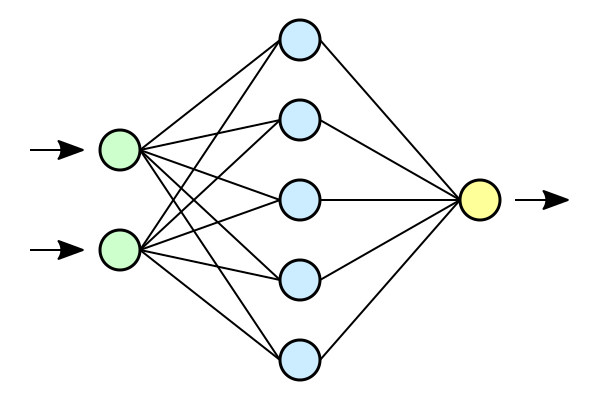
\includegraphics[width=\textwidth]{Figures/neural_network.png} 
\end{minipage} 
\begin{minipage}[t]{0.2\textwidth}
\centering
\textbf{\textcolor{red}{algorithms}} + 
\\
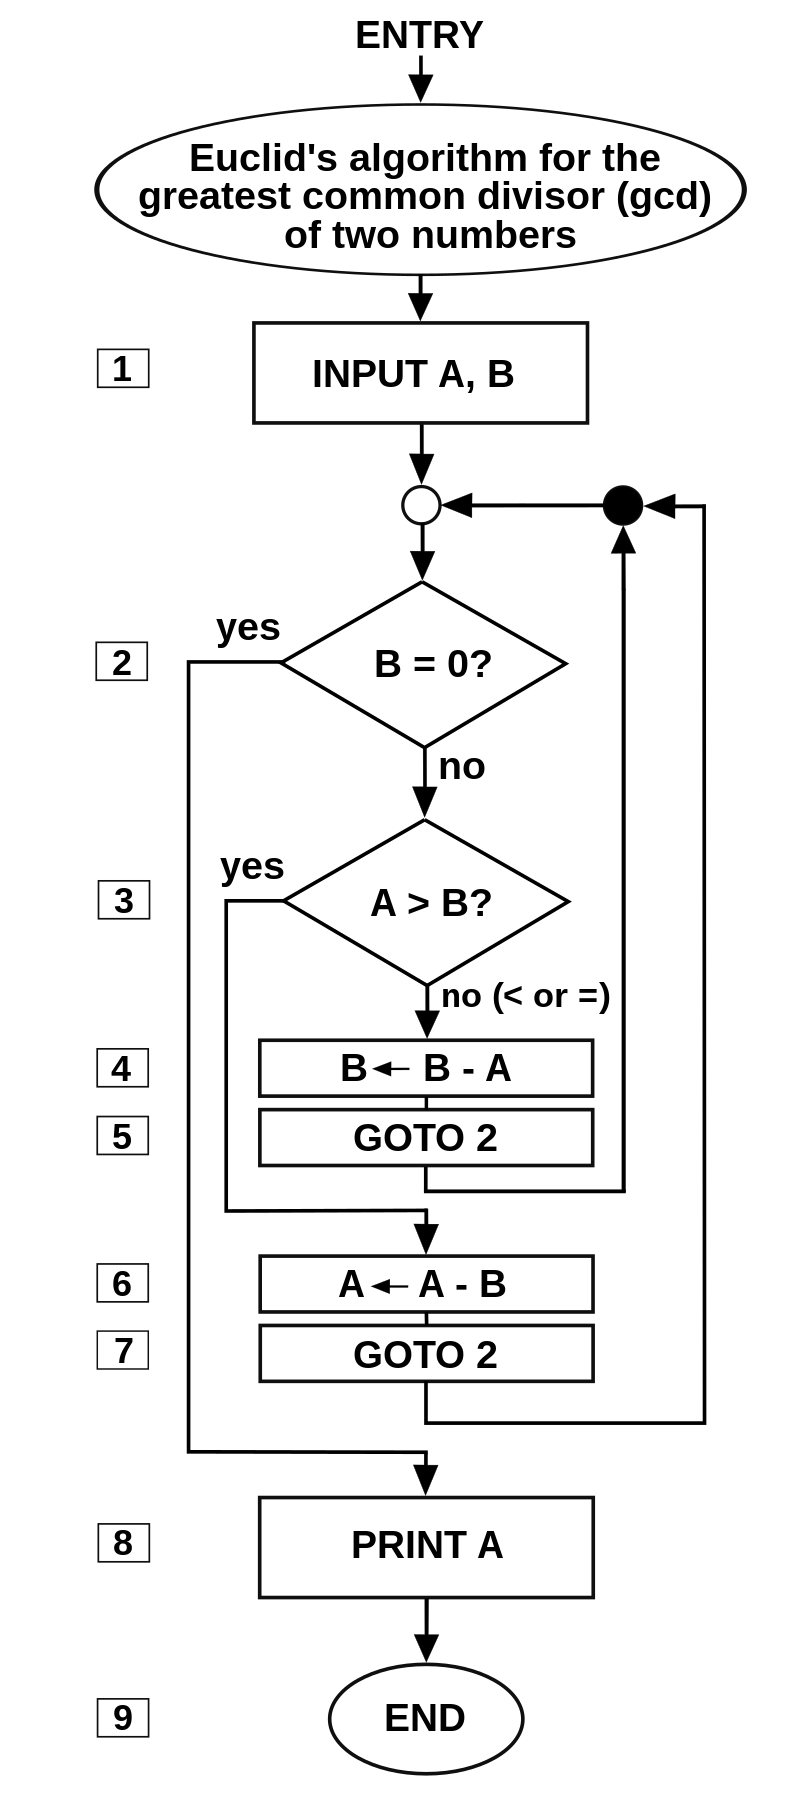
\includegraphics[width=0.5\textwidth]{Figures/algorithm.png} 
\end{minipage} 
\begin{minipage}[t]{0.2\textwidth}
\centering
data + 
\\\vskip 0.2cm

\includegraphics[width=\textwidth]{Figures/data.png} 
\end{minipage} 
\begin{minipage}[t]{0.2\textwidth}
\centering
computing power 
\\\vskip 0.2cm
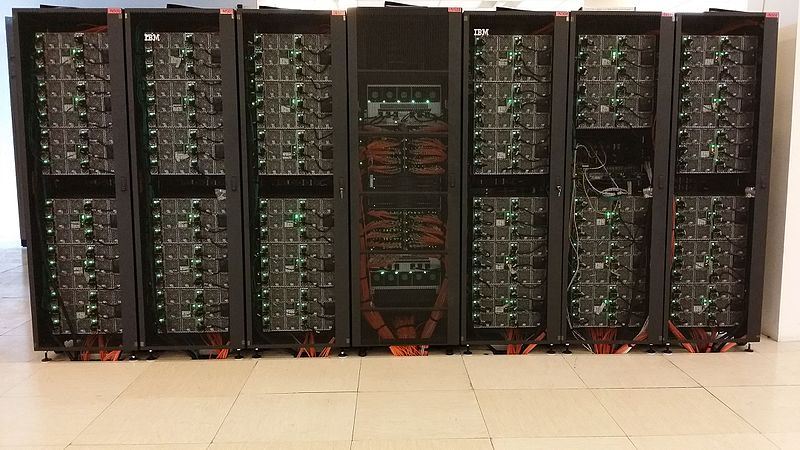
\includegraphics[width=\textwidth]{Figures/supercomputer.jpg} 
\end{minipage} 
\newpage
There are numerous conferences$^\star$ (and journals) where new optimization algorithms are presented, whether in 
\begin{itemize}
\item applied mathematics. Ex: {\scriptsize SIAM Conf. on Optimization, FGS (French-German-Swiss) workshops series, PGMO Days, \ldots}
\item computer science (including machine learning). Ex: {\scriptsize LION (Learning and Intelligent OptimizatioN conf.), EURO (EURopean Operational research soc.) conf., Optimization days, NEURIPS, \ldots}
\item or in application fields. Ex: {\scriptsize SIAM Conf. on Uncertainty Quantification (statistics), AIAA/MAO (Multidisciplinary Analysis and Optimization) or WCSMO (World Congress on Structural and Multidisciplinary Optimization) conferences (engineering), ECCOMAS (aeronautics), ICASP (civil engineering), \ldots}
\end{itemize}
\hfill($^\star$ {\scriptsize : arbitrarily listing some of the meetings I participated to} )
\newpage
Some recent algorithms are highly cited, i.e., are seen as key technological components : 
\begin{itemize}
\item NAG (\cite{nesterov1983method}, 1983, $>5500$ citations),
\item CMA-ES (\cite{hansen2001completely}, 2001, $>4100$ citations),
\item ADAGRAD (\cite{duchi2011adaptive}, 2011, $>10400$ citations),
\item RMSprop (\cite{tieleman2012lecture}, 2012, $>6000$ citations),
\item Adam (\cite{kingma2014adam}, 2014, $>113000$ citations),
\item \ldots
\end{itemize}
\end{frame}


%=======================================================================================
\begin{frame}
\frametitle{}
\centering
{\usebeamerfont*{frametitle}\usebeamercolor[fg]{frametitle} 
Optimization algorithms? 
\vskip\baselineskip
What are we talking about?
}
\end{frame}

%%%%%%%%%%%%%%%%%%%%%%%%%%%%%%%%%%%%%%%%%%%%%%%%%%%%%%%%%%%%%%%%%%
\begin{frame}[allowframebreaks]
\frametitle{The fundamental optimization problem}
\begin{minipage}{\textwidth}
\begin{minipage}{0.5\textwidth}
\centering
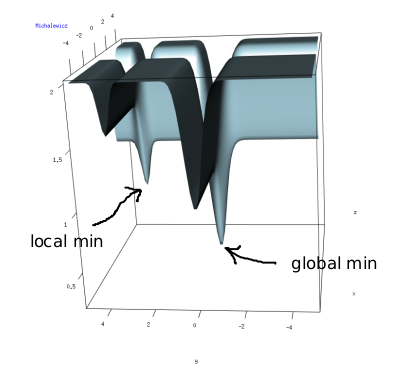
\includegraphics[width=0.9\textwidth]{michalewicz_local_global.png} \\
\vspace{-0.4cm}
{\small (2D continuous example)}
\end{minipage}
\begin{minipage}{0.45\textwidth}
Find the lowest point of a function,
\begin{equation*}
\min_{x \in \mathcal S } f(x)
\end{equation*}
\end{minipage}
\vskip\baselineskip
Looks easy on this drawing. \\
But the function is known pointwise, each evaluation costs computer time, and $\mathcal S$ may be complex (high-dimensional, non-continuous, constrained \ldots)
\end{minipage}
\newpage
\begin{minipage}{0.45\textwidth}
\centering
\begin{tikzpicture}
\node[anchor=south west,inner sep=0, outer sep=0] (contour) at (0,0) {
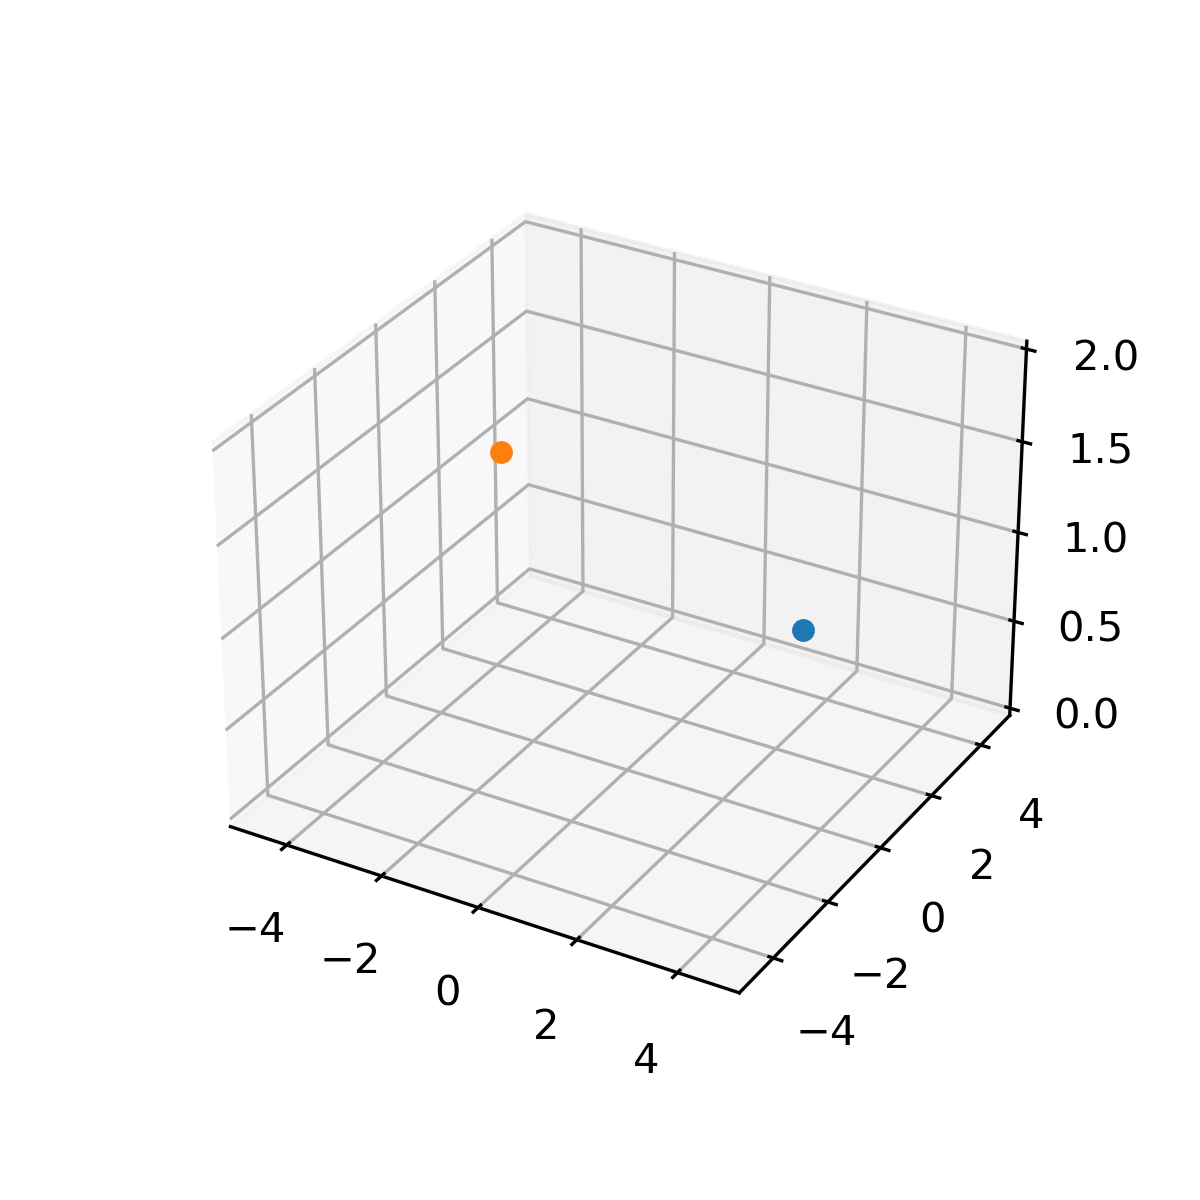
\includegraphics[width=0.9\textwidth]{two_3D_points.png}
};
\begin{scope}[x={(contour.south east)},y={(contour.north west)}]
%\draw[help lines,xstep=0.1,ystep=0.1] (0,0) grid (1,1);
\node[] (xstar) at (0.73,0.5) {$\widehat{x^\star}$};
\node[] (xprime) at (0.37,0.65) {$x'$};
\end{scope}
\end{tikzpicture}
\vspace{-0.4cm}
{\small (what the random optimizer sees)}
\end{minipage}
\hfill
\begin{minipage}{0.45\textwidth}
Random search \hfill ~\\
\noindent\rule{\textwidth}{1pt}
{\scriptsize
\begin{algorithmic}%[1]
\REQUIRE $x^\text{LB},~x^\text{UB},t^\text{max}$
\STATEx $t \leftarrow 0,~\widehat{f^\star} \leftarrow + \infty$
\WHILE{$t<t^\text{max}$}
\STATE $x' \leftarrow \mathcal U[x^\text{LB},~x^\text{UB}]\quad$ \COMMENT{uniform law}
\STATE calculate $f(x')$, $t \leftarrow t+1$
\IF{$f(x')<\widehat{f^\star}$}
\STATE $\widehat{x^\star}\leftarrow x' \quad,\quad \widehat{f^\star} \leftarrow f(x')$
\ENDIF
\ENDWHILE
\STATE \textbf{return} $\widehat{x^\star}, \widehat{f^\star}$
\end{algorithmic}
}
\vspace{-0.8\baselineskip}
\noindent\rule{\textwidth}{1pt}
\end{minipage}
\end{frame}


%%%%%%%%%%%%%%%%%%%%%%%%%%%%%%%%%%%%%%%%%%%%%%%%%%%%%%%%%%%%%%%%%
\begin{frame}[allowframebreaks]
\frametitle{Optimization = a quantitative formulation of decision}
Optimization is a way of mathematically modeling decision.
\vskip\baselineskip
\mbox{
\begin{minipage}[c]{0.3\textwidth}

\includegraphics[width=\textwidth]{decision-clipart.jpg}
\end{minipage}
\begin{minipage}[c]{0.7\textwidth}
\begin{equation*}
\min_{x \in \mathcal S} f(x)
\end{equation*}
\begin{itemize}
\item $x$ vector of decision parameters (variables)~: dimensions, investment, tuning of a machine / program, \ldots
\item $f(x)$~: decision cost, minus $\times$ performance, \ldots 
\item $\mathcal S$~: set of possible values for $x$, search space
\end{itemize}
\end{minipage}
} % end mbox
\newpage
\vskip 2cm
{\large
\begin{center}
A versatile approach to problem solving.
\vskip\baselineskip
Examples :
\end{center}
}
\end{frame}

%%%%%%%%%%%%%%%%%%%%%%%%%%%%%%%%%%%%%%%%%%%%%%%%%%%%%%%%%%%%%%%%%
\begin{frame}
\frametitle{Optimization example: aircraft global pre-design}
\begin{center}
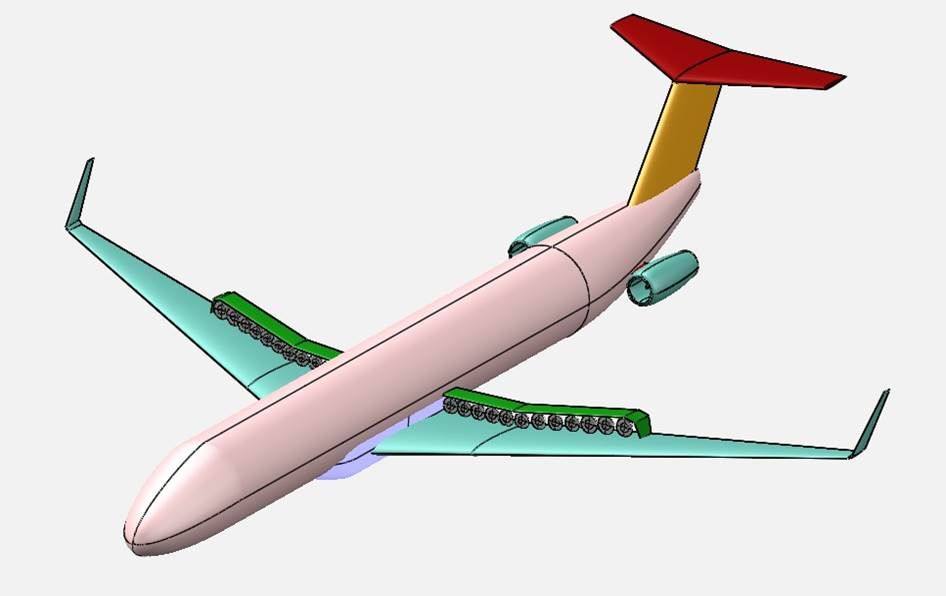
\includegraphics[width=0.5\textwidth]{aircraft_distributed_prop.png}\\
\vspace{-1cm}
{\hfill\tiny (from \cite{sgueglia2018exploration})}
\end{center}
\vskip\baselineskip
$x$ = aircraft parameters (here distributed electrical propulsion)\\
$f()$ = $-1\times$ performance metric (aggregation of $-1\times$ range, cost, take-off length, \ldots) \\
At the minimum, the design is ``optimal''.
\end{frame}


%%%%%%%%%%%%%%%%%%%%%%%%%%%%%%%%%%%%%%%%%%%%%%%%%%%%%%%%%%%%%%%%%
\begin{frame}
\frametitle{Optimization example: blade detailed design}
\begin{center}
\centering
\mbox{
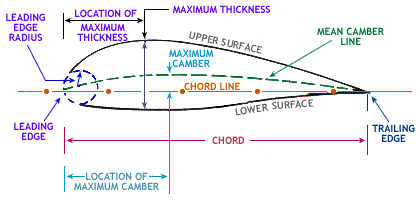
\includegraphics[width=0.33\linewidth]{Schema_Rotor}
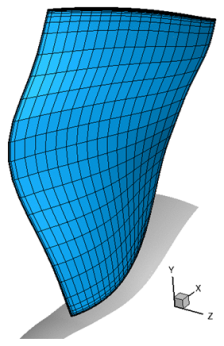
\includegraphics[width=0.13\linewidth]{blade}
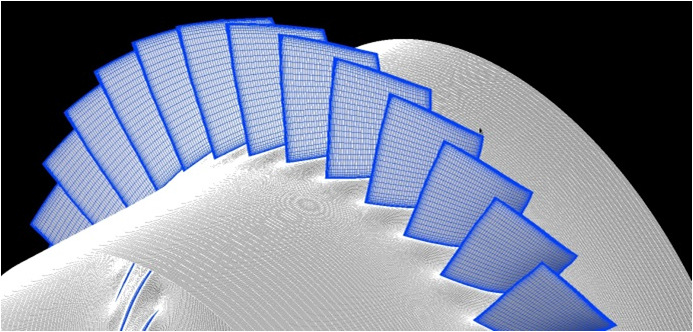
\includegraphics[width=0.33\linewidth]{rotor}
}
\end{center}
{\footnotesize
{\normalsize $x$:} The blades are described by 4 cross-sections for a total of 20 design parameters. 
\\
{\normalsize $f()$:} 5 constraints about the inlet and outlet relative flow angles, the flow speed reduction, excessive loading and the Mach number of the blade tips.
The objective function is the polytropic (compressor) efficiency. From \cite{roustant:hal-03217277}.
}
\vskip\baselineskip
Favorable application: non-intuitive design and a small gain makes a large difference.
\end{frame}

%%%%%%%%%%%%%%%%%%%%%%%%%%%%%%%%%%%%%%%%%%%%%%%%%%%%%%%%%%%%%%%%%
\begin{frame}
\frametitle{Optimization example: composite structure design}
\begin{center}
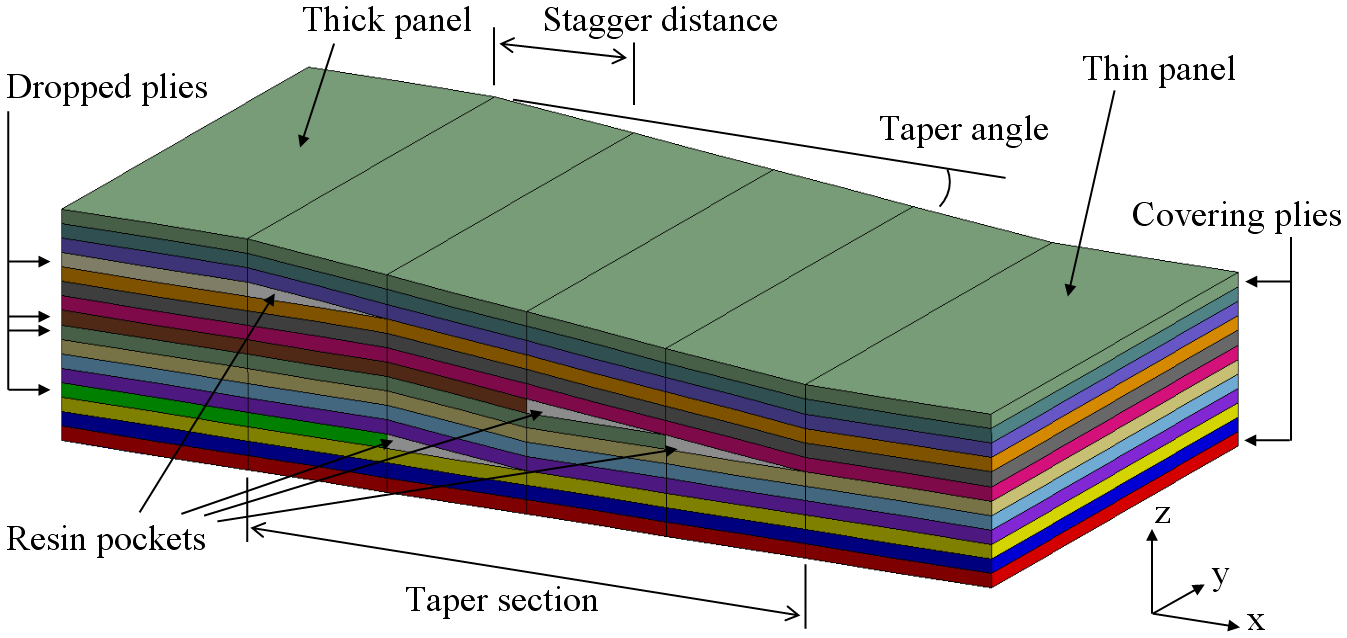
\includegraphics[width=0.7\textwidth]{ply_drop.png}
\end{center}
$x$ is the orientation of the fibers within the plies of a composite laminate and the location where the plies are dropped.
\\
$f()$ mechanical performance (stiffness, low mass, strength, stability, \ldots)
\\
Many arrangements of the $x$'s have almost equivalent performances, leading to local optima
(from \cite{irisarri2014optimal}).
\end{frame}

%%%%%%%%%%%%%%%%%%%%%%%%%%%%%%%%%%%%%%%%%%%%%%%%%%%%%%%%%%%%%%%%%
\begin{frame}
\frametitle{Optimization example: model identification}
\begin{center}
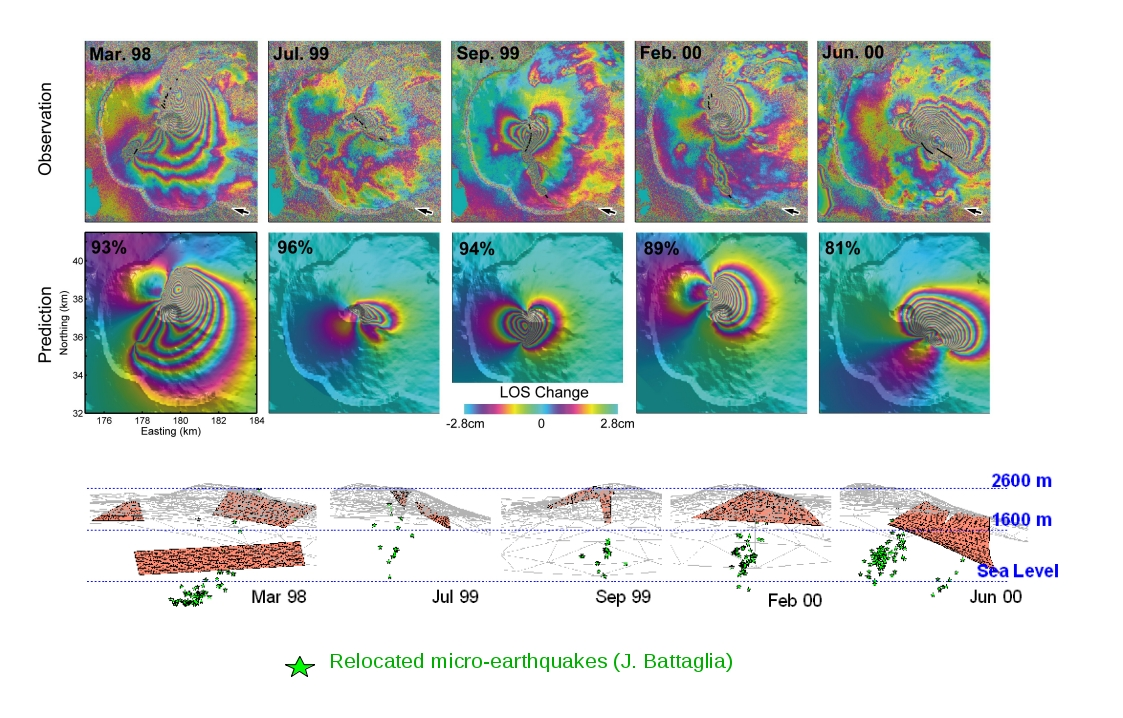
\includegraphics[width=0.7\textwidth]{piton_fournaise.jpg}\\
\vspace{-1cm}
{\hfill\tiny (from \cite{fukushima2010evolution})}
\end{center}
$x$ = dike position, geometry, internal pressure\\
$f()$ = distance between measures (from RADARSAT-1 satellite) and model (boundary elements, non trivial computation)\\
At the minimum, the model best matches measurements and should correspond to the underground phenomenon.
\end{frame}

%%%%%%%%%%%%%%%%%%%%%%%%%%%%%%%%%%%%%%%%%%%%%%%%%%%%%%%%%%%%%%%%%
\begin{frame}
\frametitle{Optimization example: wind farm layout}
\begin{center}
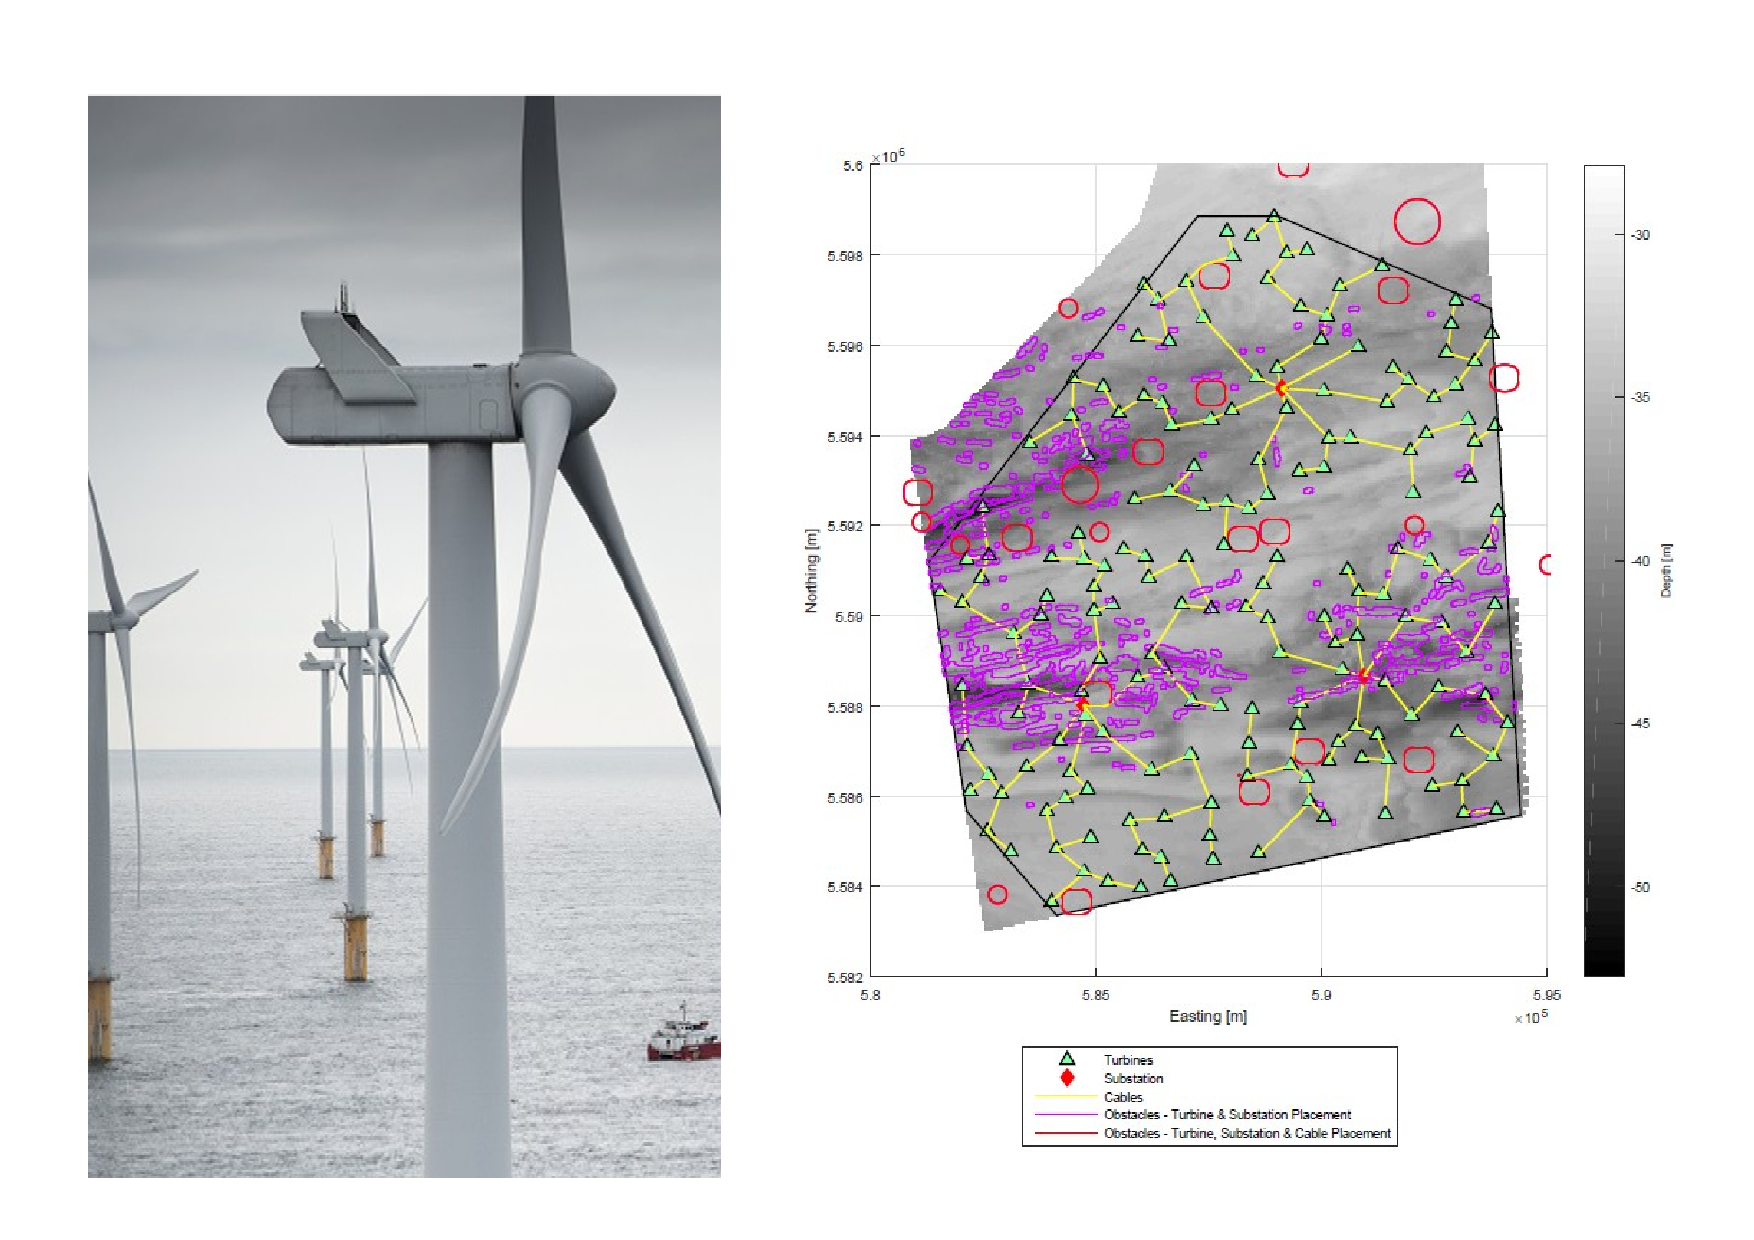
\includegraphics[width=0.7\textwidth]{wind_farm_model.pdf}
\end{center}
$x$ = position and characteristics of the wind mill, electrical network.
$f()$ = cost aggregated with -1 $\times$ average power production.
\end{frame}

%%%%%%%%%%%%%%%%%%%%%%%%%%%%%%%%%%%%%%%%%%%%%%%%%%%%%%%%%%%%%%%%%
\begin{frame}
\frametitle{Optimization example: image denoising}
\vspace{-0.5cm}
\begin{equation*}
\begin{split}
\min_x f(x) \quad,\quad & f(x) = \frac{1}{2}\sum_{i=1}^{N_{\text{pixels}}} (y_i - x_i)^2 + 
\lambda \sum_{i=1}^{N_{\text{pixels}}} \sum_{j \text{ near } i} \lvert x_i - x_j \rvert \\
& \lambda \ge 0 \quad\text{regularization constant}
\end{split}
\end{equation*}
\begin{center}
\begin{minipage}[t]{0.2\textwidth}

\includegraphics[width=\textwidth]{c_clean.png} \\
{\small target image}
\end{minipage}
\hfill
\begin{minipage}[t]{0.2\textwidth}

\includegraphics[width=\textwidth]{c_noisy.png} \\
{\small \mbox{noisy (observed)} $= y_i$'s}
\end{minipage}
\hfill
\begin{minipage}[t]{0.2\textwidth}

\includegraphics[width=\textwidth]{c_denoised.png} \\
{\small \mbox{denoised (optimized)} $=x^\star$}
\end{minipage}
\mbox{\quad}
\end{center}
{\scriptsize (from \cite{ravikumar17}) \hfill}
\end{frame}

%%%%%%%%%%%%%%%%%%%%%%%%%%%%%%%%%%%%%%%%%%%%%%%%%%%%%%%%%%%%%%%%%
\begin{frame}
\frametitle{Optimization example: neural net learning}
\begin{minipage}{0.5\textwidth}
$x$ = neural network (NN) weights and biases
\vskip\baselineskip
$f()$ = an error of the NN predictions w.r.t. data (a loss function)
\end{minipage}
\hfill
\begin{minipage}{0.4\textwidth}
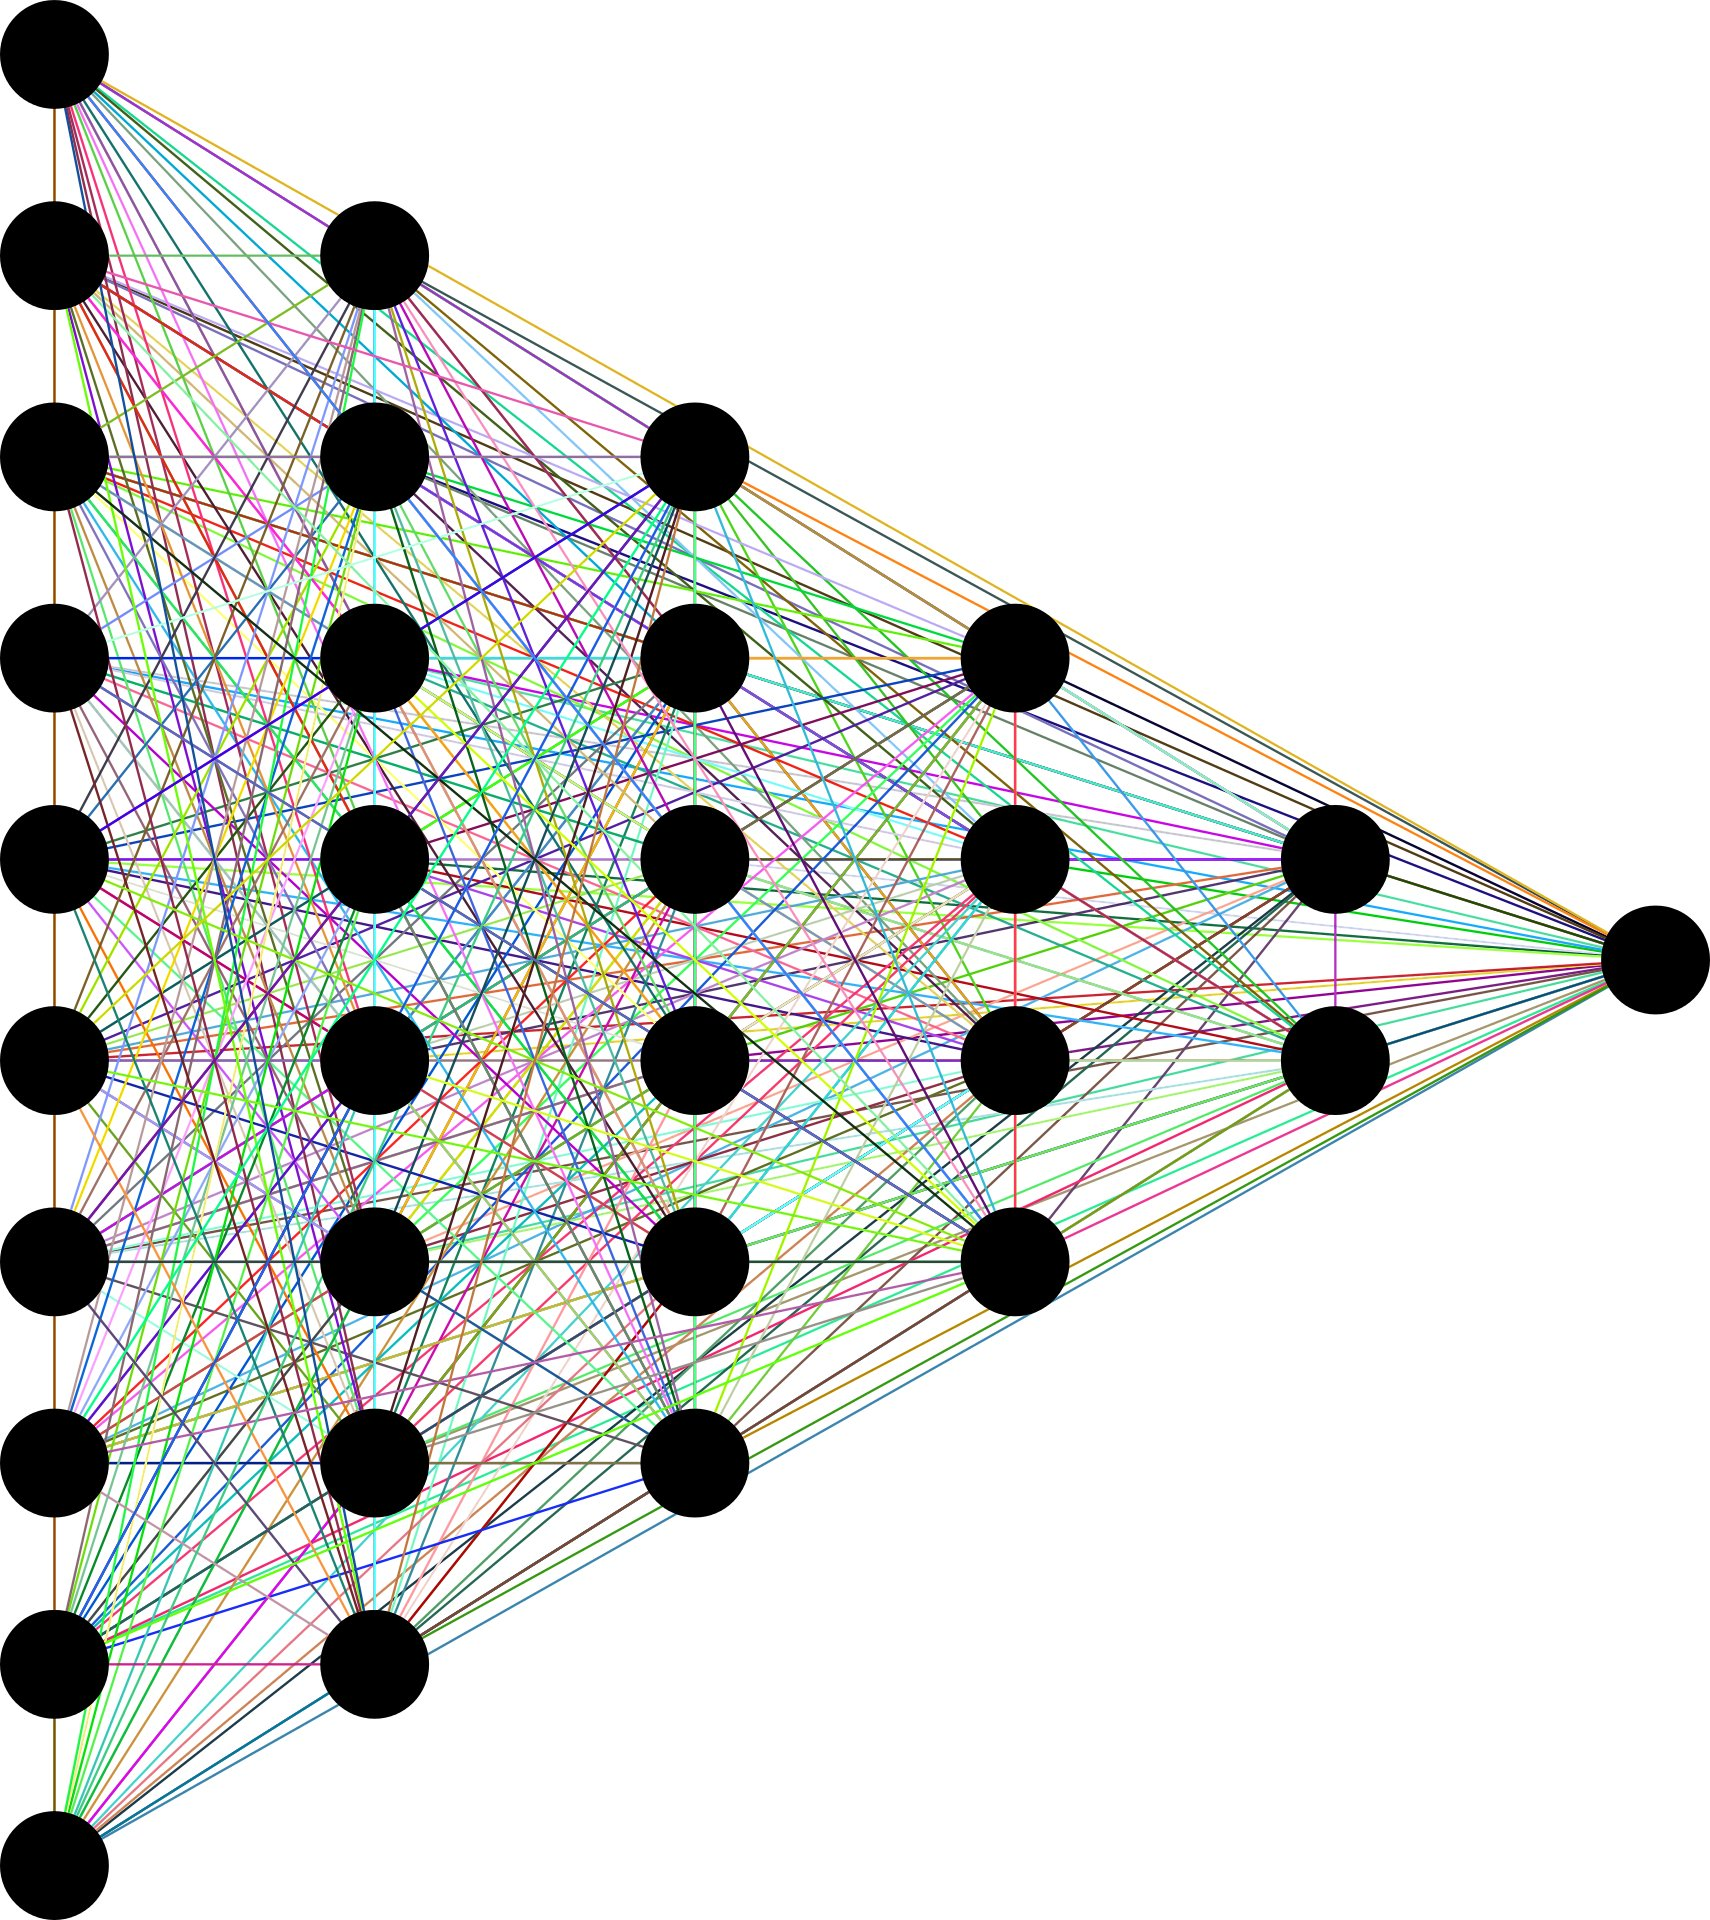
\includegraphics[width=\textwidth]{neuralnetwork_CC0_public_domain.jpg} \\
{\tiny from \url{techxplore.com/news/2020-11-neural-network.html}, CC0 public domain \par}
\end{minipage}
\end{frame}


%%%%%%%%%%%%%%%%%%%%%%%%%%%%%%%%%%%%%%%%%%%%%%%%%%%%%%%%%%%%%%%%%
\begin{frame}
\frametitle{An utopia ? Humans in the loop}
Optimization as a mathematical model for decision
\vskip\baselineskip
\mbox{
\begin{minipage}[c]{0.2\textwidth}

\includegraphics[width=\textwidth]{decision-clipart.jpg}
\end{minipage}
\begin{minipage}[c]{0.7\textwidth}
\begin{equation*}
\min_{x \in \mathcal S} f(x)
\end{equation*}
\end{minipage}
} % end mbox
\vskip\baselineskip
Don't forget the human in the loop ! 
\begin{itemize}
\item In \cite{tsoukias2008decision}, broader framework (model of the human rationality) $\Rightarrow$ decision \alert{aiding} theory.
\item Multi-Disciplinary Optimization \cite{brevault2020aerospace} as an attempt to model interacting disciplines.
\item Human systems are complex, not easy to model.
\end{itemize}
\begin{block}{}
Here, modest and practical goal : optimization as a (fascinating) \alert{tool}.
\end{block}
\end{frame}

%=======================================================================================
\begin{frame}
\frametitle{}
\centering
{\usebeamerfont*{frametitle}\usebeamercolor[fg]{frametitle} 
Historical and epistemological hints
\vskip\baselineskip
}
\end{frame}


%%%%%%%%%%%%%%%%%%%%%%%%%%%%%%%%%%%%%%%%%%%%%%%%%%%%%%%%%%%%%%%%%
\begin{frame}%[allowframebreaks]
\frametitle{Emergence conditions}
Optimization algorithms have become a scientific subject of its own when the problem to solve has been decomposed into 
\begin{itemize}
\item a real object to optimize,
\item a space of representations $\mathcal S$ where $x$ is chosen,
\item a model of the object valid for each representation, $m(x)$,
\item a performance measure $f(m(x))$,
\item a motion principle (the optimization algorithm).
\end{itemize}
\vskip\baselineskip
{\footnotesize
Ex. in engineering: an object to design, $x$ CAD parameters, $m(x)$ a finite elements model, $f()$ a compromise between -strength and cost. \\
Ex. in machine learning: a neural network to learn, $x$ the weights, $m(x)$ the responses of the network over a certain data base, $f()$ the loss function.
}
\end{frame}

%=======================================================================================
\begin{frame}
\frametitle{The decomposition principle}
\begin{block}{}
Elements of scientific knowledge appear when a problem is sufficiently decomposed.
\end{block}
\begin{itemize}
\item Close to Descartes' 2nd Rule in Discourse on the Method : ``Divide each difficulty into as many parts as is feasible and necessary to resolve it''
(but applied to a scientific domain).
\end{itemize}
In the case of optimizers:
\begin{itemize}
\item A space-time generalized decomposition in the sense of Bernard Guy \cite{guyTempsEspace}, where time is related to the motion of the optimizer.
\item When applied to machine learning, optimizers are part of a constructivist system \cite{sarkar2016constructivist}: learnings occurs by the interaction between perception (ideas, = simulated actions) and action, new experience, in a trial and error process guided by the optimizer.
\end{itemize}
\end{frame}

%=======================================================================================
\begin{frame}
\frametitle{}
~
\vfill
{\large
The emergence of optimization algorithms occured after World War II.\\
Optimization problems were solved before, but in a unified manner. \\
\vskip\baselineskip
Examples:
}
\vfill
~
\end{frame}

%=======================================================================================
\begin{frame}
\frametitle{da Vinci's flying machine}
\begin{center}
Design for a flying machine, Leonardo da Vinci, 1488.
\vskip\baselineskip
\begin{minipage}{0.8\textwidth}
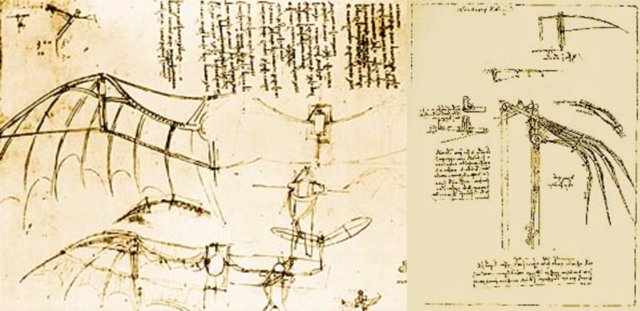
\includegraphics[width=\textwidth]{Mechanical-Wing-Devices-Leonardo-da-Vinci-ca-1485-From-Miller-2008_W640.jpg} \\
\end{minipage}
\end{center}
\end{frame}

%=======================================================================================
\begin{frame}
\frametitle{Hooke's arch}
\begin{minipage}{0.4\textwidth}
Optimization of an arch.\\
Hooke's theorem (1675) :\\
``As hangs the flexible chain, so but inverted will stand the rigid arch.''
\\
\begin{center}
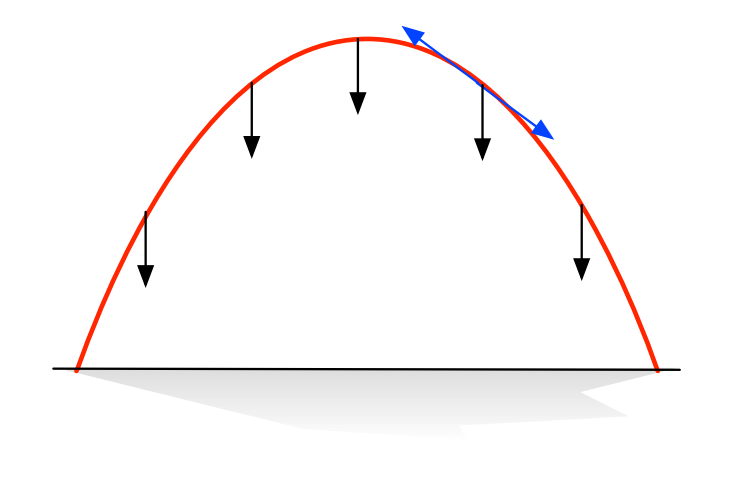
\includegraphics[width=0.65\textwidth]{arche.png}
\end{center}
\end{minipage}
\hfill
\begin{minipage}{0.4\textwidth}
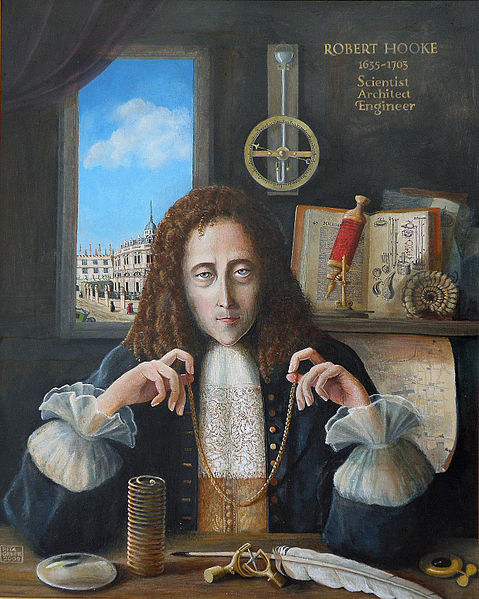
\includegraphics[width=\textwidth]{Robert-Hooke.jpeg} \\
{\tiny 
Robert Hooke holding a chain that forms a catenary curve. 
Image by Rita Greer. Licensed under Free Art License 1.3, via Wikimedia Commons.}
\end{minipage}
\end{frame}

%=======================================================================================
\begin{frame}
\frametitle{The Brachistochrone curve}
\begin{minipage}{\textwidth}
Minimize time to go from a point to a lower point with a frictionless ball under the action of gravity. 
\vskip\baselineskip
Posed and solved by Johann Bernoulli in 1696.
\end{minipage}
\begin{center}
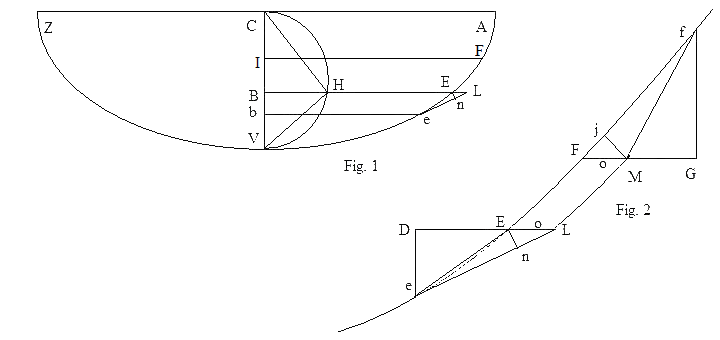
\includegraphics[width=0.7\textwidth]{Bernoulli_Challenge_to_Newton_1.png} \\
\end{center}
\end{frame}

%=======================================================================================
\begin{frame}
\frametitle{Millau's viaduct}
\begin{minipage}{\textwidth}
Michel Virlogeux, main designer:\\  
``The preliminary design of Millau's viaduct was first scribbled on a restaurant tablecloth and it was quite right. Computations then confirmed the ideas and fine tuned the details.'' 
\end{minipage}
\vskip\baselineskip
\mbox{
\begin{minipage}{0.4\textwidth}
{\scriptsize (talk at Maison de la Mécanique, Courbevoie, France, around 2005. \\
Millau's viaduct is currently the tallest bridge in the world.)}
\end{minipage}
\begin{minipage}{0.6\textwidth}
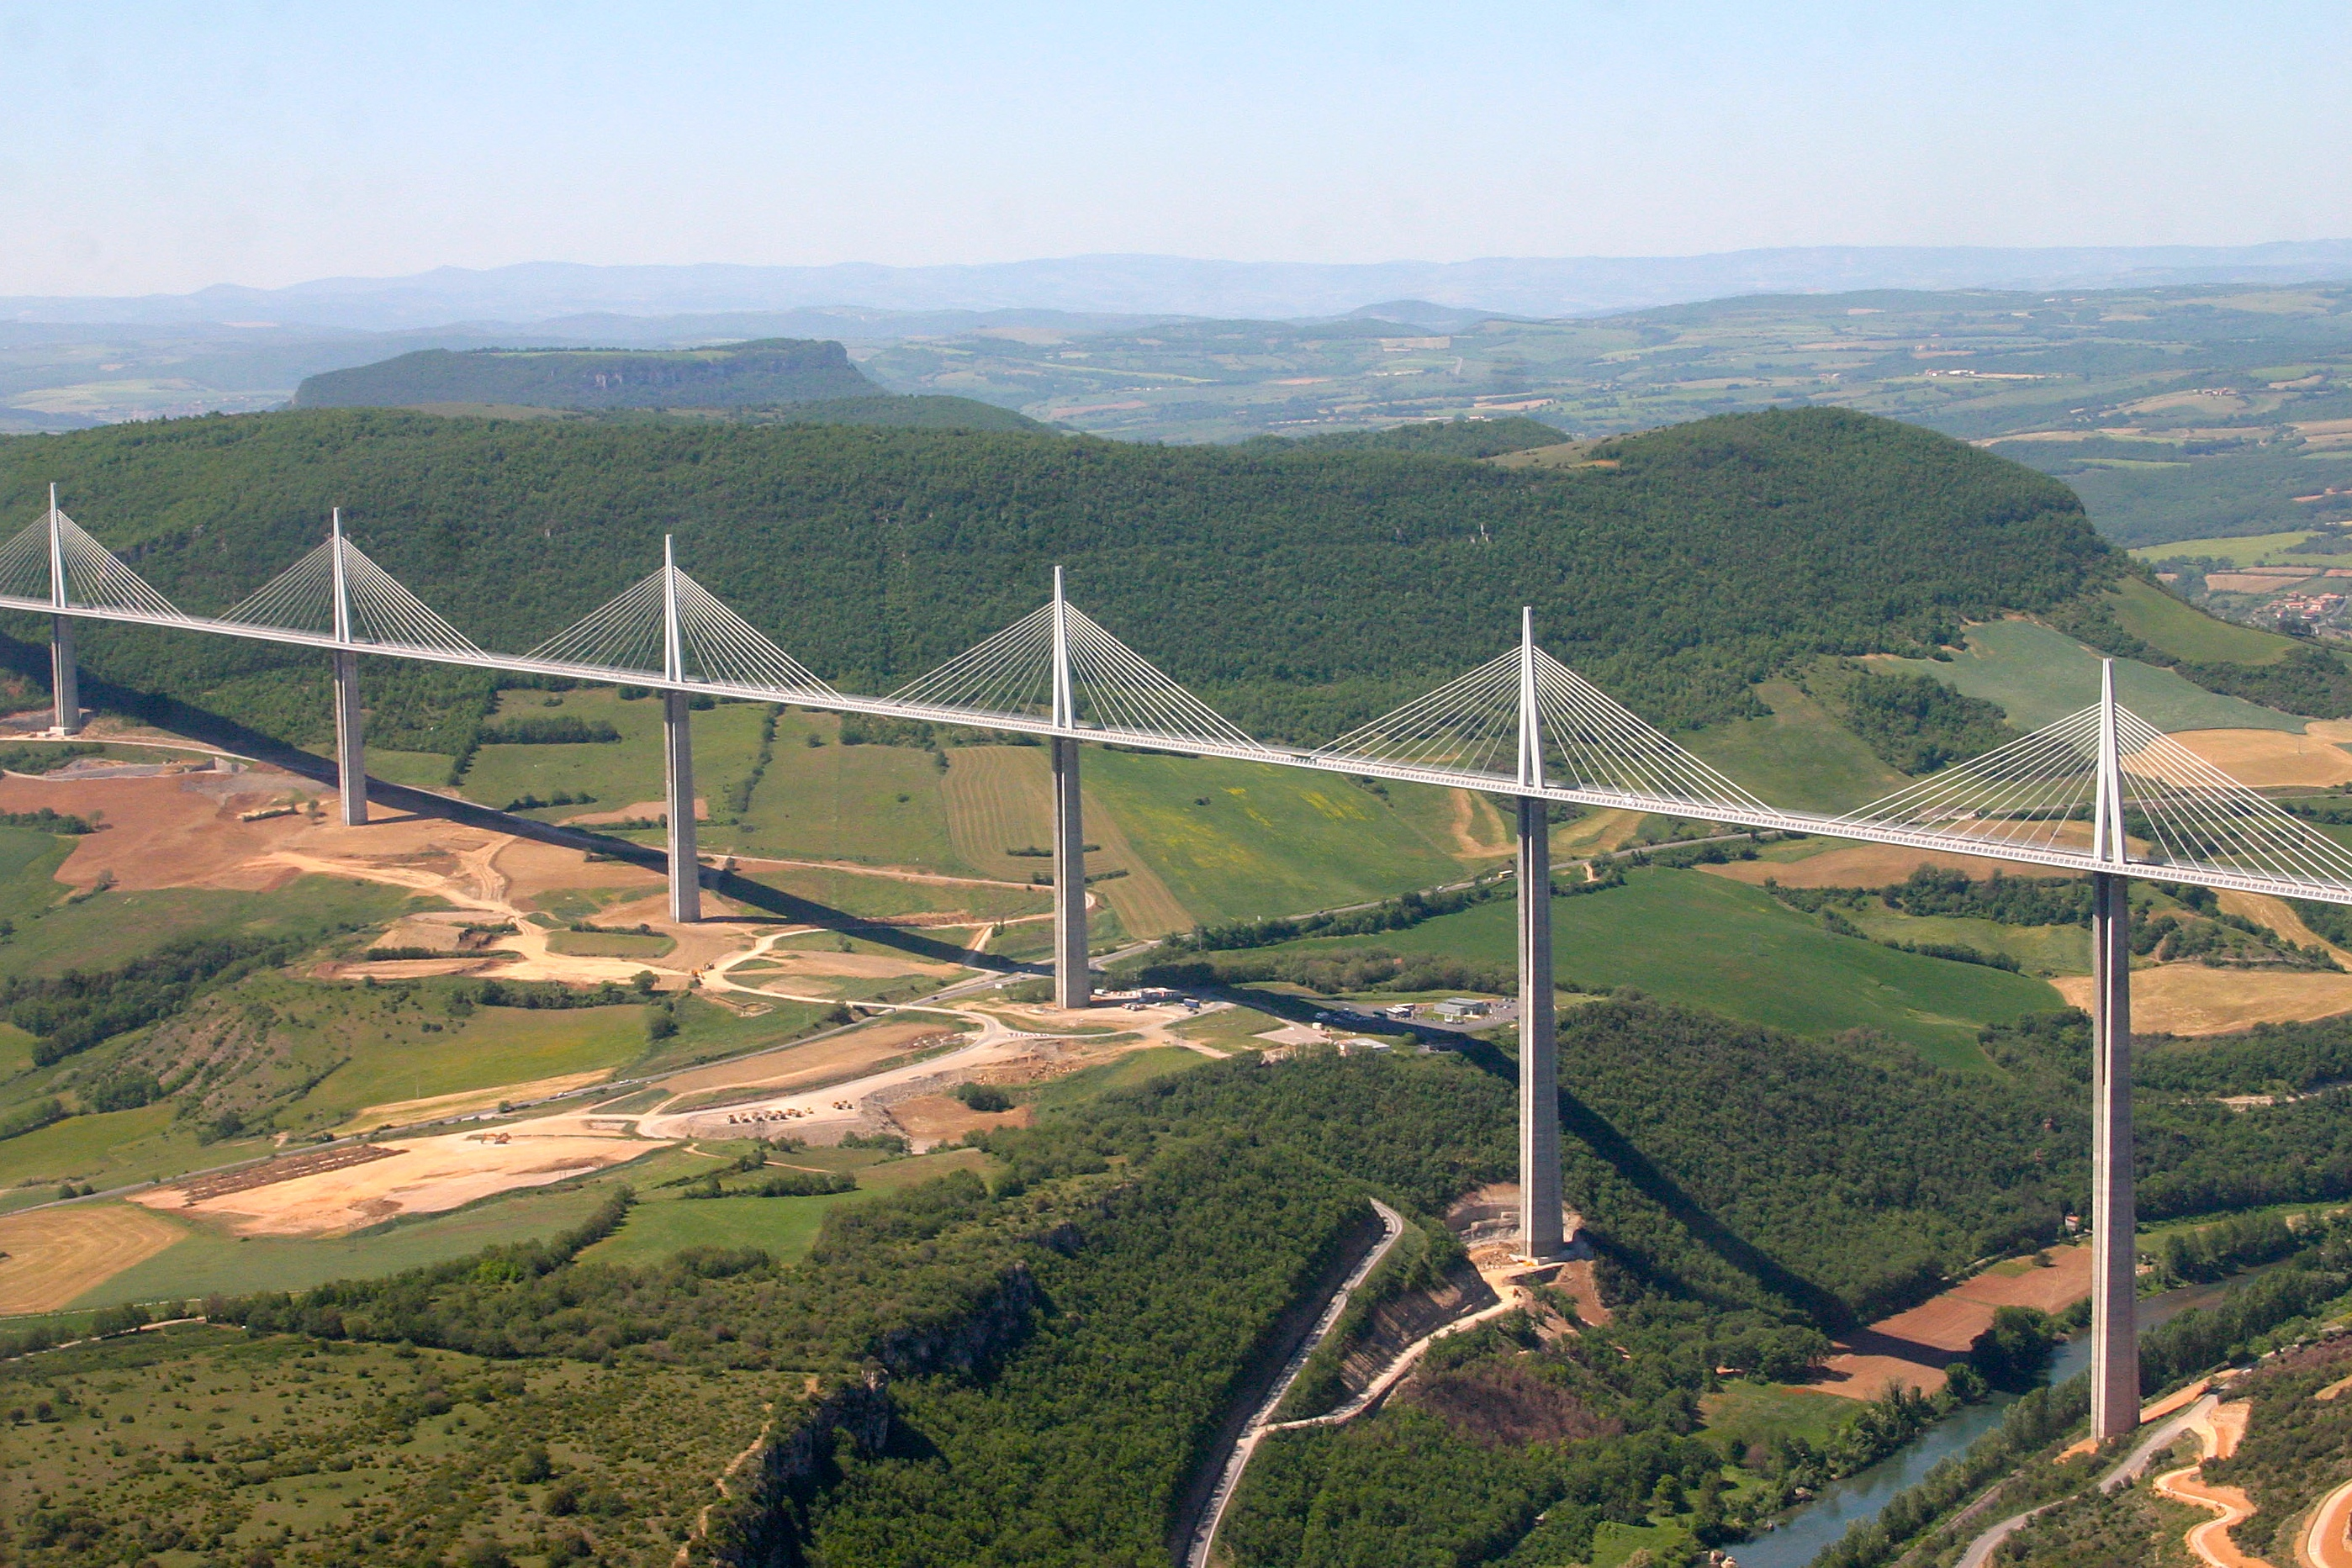
\includegraphics[width=\textwidth]{ViaducdeMillau.jpg} 
\end{minipage}
}
\end{frame}

%=======================================================================================
\begin{frame}
\frametitle{The first optimization algorithms}
They appeared after World War II, thanks to the first computers and a sufficient scientific maturity (cf. decomposition principle).
\begin{itemize}
\item The Steepest Descent Algorithm was formulated in its general form in 1944 by Haskell B. Curry \cite{curry1944method} after initial ideas by Augustin Louis Cauchy in 1847 applied to astronomical equations solving \cite{lemarechal2012cauchy}.
\item The Simplex Algorithm for solving linear problems was proposed around 1947 by George B. Dantzig \cite{dantzig1955generalized}.
\item The Response Surface Method for approximating $f$ by a quadratic function throughout $\mathcal S$ was proposed by George E. P. Box and Kenneth B. Wilson in 1951 \cite{box1951experimental}.
\end{itemize}
\end{frame}


%=======================================================================================
\begin{frame}[allowframebreaks]
\frametitle{Today's optimization algorithms}
{\footnotesize (the discussion is voluntarily kept as short and non-technical as possible)}
\vskip\baselineskip
\begin{itemize}
\item Proven rapid (in polynomial time or super-linear) convergence for convex problems: cf. improved gradient descents such as BFGS (accounting for curvatures) and NAG \cite{nesterov1983method}.
\item Algorithms adapted to stochastic functions (variants of stochastic gradients such as Adam \cite{kingma2014adam}).
\item Algorithms using stochastic choices (e.g., CMA-ES \cite{hansen2001completely}).
\item[$\Rightarrow$] Recognition of the importance of uncertainties, for which randomness is both an ingredient and a cure.
\newpage
\item Algorithms building models of the function (Bayesian optimization, \cite{ExpectedImprovement}) or of their validity domain (DFO, \cite{audet2017derivative}).
\item A lot of specialized versions: with/without constraints, for multiple objectives, with discrete and/or continuous variables, depending on the numerical cost of the function and the number of variables, \ldots
\end{itemize}
\end{frame}

%%%%%%%%%%%%%%%%%%%%%%%%%%%%%%%%%%%%%%%%%%%%%%%%%%%%%%%%%%%%%%%%%
\begin{frame}
\frametitle{An utopia ? Computational limitations}
The fundamental problem, $ \min_{x \in \mathcal S } f(x) $,
is rarely solved in practice because the optimizer stops its iterations earlier (computational limitation).\\
\begin{minipage}{0.4\textwidth}
In machine learning, when optimizing the loss function with a stochastic gradient, a situation in between the red and the blue convergences occurs. Yet, ``it works''.
\end{minipage}
\hfill
\begin{minipage}{0.55\textwidth}
\includegraphics[width=\textwidth]{tooHigh.png} 
\end{minipage}
\end{frame}

%%%%%%%%%%%%%%%%%%%%%%%%%%%%%%%%%%%%%%%%%%%%%%%%%%%%%%%%%%%%%%%%%
\begin{frame}
\frametitle{An utopia ? Bounded rationality}
(cf. Herbert A. Simon)
\vskip\baselineskip
what's the point of accurately solving the problem since the formulation will always be imperfect? 
\begin{itemize}
\item The model, $m()$ is inaccurate.
\item Some variables are missing (some dimensions of $\mathcal S$).
\item Other objectives (utilities, $f_1(),\ldots,f_N()$, $N$ potentially infinite) exist as well.
\end{itemize}
\end{frame}

%%%%%%%%%%%%%%%%%%%%%%%%%%%%%%%%%%%%%%%%%%%%%%%%%%%%%%%%%%%%%%%%%
\begin{frame}
\frametitle{Some current challenges}
Optimization algorithms are a recent research domain. Still a lot to do!
\begin{itemize}
\item Properly testing and characterizing optimization algorithms is needed. The relationship between the best optimizer and the problem is complex. Initial work in {\scriptsize \cite{hansen2021coco,bosse2012relative,kerschke2019automated}}.
\item Handling uncertainties in optimization problems is fundamental. An active sub-domain. Recent bibliography in {\scriptsize \cite{pelamatti2022coupling}}.
\item The curse of dimensionality (with limited computations). Cf. e.g. {\scriptsize\cite{binois:hal-03419959}}.
\item Less common types of variables : mixed (discrete-continuous, e.g.,{\scriptsize\cite{cuesta2022comparison}}), functional, or graph variables.
\item Massively parallel, asynchronous, fault tolerant optimizers.
\end{itemize}
\end{frame}

\section{Bibliography}

%=======================================================================================
\begin{frame}[allowframebreaks]
\frametitle{References}
\scriptsize
%\vspace{-1.cm}
%\setbeamertemplate{bibliography item}{[\theenumiv]} % to have numbers in biblio with beamer
%   \bibliographystyle{plain}
   \bibliographystyle{apalike}
   \bibliography{biblio}
\end{frame}

\end{document}

